\documentclass[12pt,a4paper,twoside]{report}
% -------------------------------------------------------------------- %
% Pacotes

\usepackage[utf8]{inputenc}
\usepackage[T1]{fontenc}
\usepackage[brazil]{babel}
\usepackage[fixlanguage]{babelbib}
\usepackage[pdftex]{graphicx}      % usamos arquivos pdf/png como figuras
\usepackage{setspace}              % espaçamento flexvel
\usepackage{indentfirst}           % indentação do primeiro parágrafo
\usepackage{makeidx}               % índice remissivo
\usepackage[nottoc]{tocbibind}     % acrescentamos a bibliografia/indice/conteudo no Table of Contents
\usepackage{courier}               % usa o Adobe Courier no lugar de Computer Modern Typewriter
\usepackage{type1cm}               % fontes realmente escaláveis
\usepackage{titletoc}
\usepackage{ucs}
\usepackage[font=small,format=plain,labelfont=bf,up,textfont=it,up]{caption}
\usepackage[usenames,svgnames,dvipsnames]{xcolor}
\usepackage[a4paper,top=2.54cm,bottom=2.0cm,left=2.0cm,right=2.54cm]{geometry} % margens
\usepackage{amsmath} 

\usepackage[pdftex,plainpages=false,pdfpagelabels,pagebackref,colorlinks=true,citecolor=DarkGreen,
linkcolor=NavyBlue,urlcolor=DarkRed,filecolor=green,bookmarksopen=true]{hyperref} % links coloridos
\usepackage[all]{hypcap}                % soluciona o problema com o hyperref e capítulos
\usepackage[square,sort,nonamebreak,comma]{natbib}  % citação bibliográfica alpha
\fontsize{60}{62}\usefont{OT1}{cmr}{m}{n}{\selectfont}
\usepackage{upquote}                    % formata apóstrofes '
\usepackage{textcomp}

% Para formatar corretamente as URLs
\usepackage{url}
% -------------------------------------------------------------------- %
% Cabeçalhos similares ao TAOCP de Donald E. Knuth
\usepackage{fancyhdr}
\pagestyle{fancy}
\fancyhf{}
\renewcommand{\chaptermark}[1]{\markboth{\MakeUppercase{#1}}{}}
\renewcommand{\sectionmark}[1]{\markright{\MakeUppercase{#1}}{}}
\renewcommand{\headrulewidth}{0pt}

% -------------------------------------------------------------------- %
\graphicspath{{./imagens/}}        % caminho das figuras
\frenchspacing                     % arruma o espaço: id est (i.e.) e exempli gratia (e.g.)
\urlstyle{same}                    % URL com o mesmo estilo do texto e no mono-spaced
\makeindex                         % para o índice remissivo
\raggedbottom                      % para no permitir espaços extras no texto
\fontsize{60}{62}\usefont{OT1}{cmr}{m}{n}{\selectfont}
\cleardoublepage
\normalsize

% -------------------------------------------------------------------- %
% Cores para formatação de código
\usepackage{color}
\definecolor{vermelho}{rgb}{0.6,0,0} % para strings
\definecolor{verde}{rgb}{0.25,0.5,0.35} % para comentários
\definecolor{roxo}{rgb}{0.5,0,0.35} % para palavras-chaves
\definecolor{azul}{rgb}{0.25,0.35,0.75} % para strings
\definecolor{cinza-claro}{gray}{0.95}
% -------------------------------------------------------------------- %
% Opções de listagem usados para o código fonte
% Ref: http://en.wikibooks.org/wiki/LaTeX/Packages/Listings



\usepackage{listings}           % para formatar código-fonte (ex. em Java)


\lstset{ %
language=[Objective]Caml,  % seleciona a linguagem do código (aqui em lstlang0.sty
basicstyle=\footnotesize\ttfamily, % o tamanho da fonte usado no código
commentstyle=\color{verde}\bfseries,  % formatação de comentários
stringstyle=\color{azul},    % formatação de strings
upquote=true,
numbers=left,                   % onde colocar os números de linha
numberstyle=\tiny,  % o tamanho da fonte usada para a numeração das linhas
stepnumber=1,                   % o intervalo entre dois números de linhas. Se for 1, numera cada uma.
numbersep=5pt,                  % how far the line-numbers are from the code
showspaces=false,               % show spaces adding particular underscores
showstringspaces=false,         % underline spaces within strings
showtabs=false,                 % show tabs within strings adding particular underscores
keywordstyle=\color{roxo}\bfseries,
keywordstyle=[1]\color{roxo}\bfseries,
keywordstyle=[2]\color{verde}\bfseries,
%        keywordstyle=[3]\textbf,    %
%        keywordstyle=[4]\textbf,   \sqrt{\sqrt{}} %
frame=b,                   % adds a frame around the code
framerule=0.6pt,
tabsize=2,                      % sets default tabsize to 2 spaces
captionpos=t,                   % sets the caption-position to top
breaklines=true,                % sets automatic line breaking
breakatwhitespace=false,        % sets if automatic breaks should only happen at whitespace
escapeinside={\%*}{*)},         % if you want to add a comment within your code
backgroundcolor=\color[rgb]{1.0,1.0,1.0}, % choose the background color.
rulecolor=\color[rgb]{0.8,0.8,0.8},
extendedchars=true,
xleftmargin=10pt,
xrightmargin=10pt,
framexleftmargin=10pt,
framexrightmargin=10pt,
literate={â}{{\^{a}}}1  % para formatar corretamente os acentos do Português ao usar utf8
    {ê}{{\^{e}}}1
    {ô}{{\^{o}}}1  
    {Â}{{\^{A}}}1
    {Ê}{{\^{E}}}1
    {Ô}{{\^{O}}}1
    {á}{{\'{a}}}1
    {é}{{\'{e}}}1
    {í}{{\'{i}}}1
    {ó}{{\'{o}}}1
    {ú}{{\'{u}}}1
    {Á}{{\'{A}}}1
    {É}{{\'{E}}}1
    {Í}{{\'{I}}}1
    {Ó}{{\'{O}}}1
    {Ú}{{\'{U}}}1
    {à}{{\`{a}}}1
    {À}{{\`{A}}}1
    {ã}{{\~{a}}}1
    {õ}{{\~{o}}}1
    {Ã}{{\~{A}}}1
    {Õ}{{\~{O}}}1
    {ç}{{\c{c}}}1
    {Ç}{{\c{C}}}1
    {ü}{{\"u}}1
    {Ü}{{\"U}}1
}

\renewcommand{\lstlistingname}{Listagem}
\renewcommand{\lstlistlistingname}{Lista de Listagens}

% Definição de novos estilos
\lstdefinestyle{Bash}
    {language=bash,frame=single,numbers=none,basicstyle=\footnotesize\ttfamily,
     morekeywords={cp,mkdir,sudo,tar}}

% Definição de novos ambientes
\lstnewenvironment{terminal}
  {\lstset{style=Bash}}
  {}

\lstnewenvironment{ocaml}
  {\lstset{basicstyle=\scriptsize\ttfamily,
           frame=single,
           frameround=tttt,
           framerule=2pt,
           numbers=none,
           rulecolor=\color{Salmon}}}
  {}

\lstnewenvironment{xml}
   {\lstset{language=XML,frame=single,numbers=none}}
   {}

\lstnewenvironment{interprete}
  {\lstset{frame=single,
            frameround=tttt,
            numbers=none,
            basicstyle=\ttfamily,
            framerule=2pt,
            rulecolor=\color{CadetBlue}}}
  {}
% Formata o caption da listagem
% \DeclareCaptionFont{blue}{\color{blue}} 

% \captionsetup[lstlisting]{singlelinecheck=false, labelfont={blue}, textfont={blue}}
\usepackage{caption}
\DeclareCaptionFont{white}{\color{white}}
\DeclareCaptionFormat{listing}{\colorbox[cmyk]{0.43, 0.35, 0.35,0.01}{\parbox{\textwidth}{\hspace{15pt}#1#2#3}}}
\captionsetup[lstlisting]{format=listing,labelfont=white,textfont=white, singlelinecheck=false, margin=0pt, font={bf,footnotesize}}

\newcommand{\ListingsPath}{./codigos}
% Inclui o nome do arquivo como Caption 
\newcommand{\filelisting}[2][]{%
    \lstinputlisting[caption={\texttt{\detokenize{#2}}},#1]{\ListingsPath/#2}%
}

% ---------------------------------------------------------------------------- %

% ---------------------------------------------------------------------------- %

\title{Construção de um compilador de MiniC para LLVM usando Objective Caml}
\date{}
\author{Leandro de Medeiros Ferreira \\
\texttt{\small \url{leandromf@live.com}}\\
\vspace{10cm} \\
Faculdade de Computação \\
Universidade Federal de Uberlândia
}
\date{\today}

%\includeonly{cap-clojure,magical,short}
\begin{document}
  \maketitle
% -------------------------------------------------------------------- %
% Listas de figuras, tabelas e códigos criadas automaticamente
\listoffigures            
\listoftables            
\lstlistoflistings
% -------------------------------------------------------------------- %

% -------------------------------------------------------------------- %
% Sumário
\tableofcontents    

% Capítulos do trabalho

% cabeçalho para as páginas de todos os capítulos
\fancyhead[RE,LO]{\thesection}

%\singlespacing              % espaçamento simples
\setlength{\parskip}{0.15in} % espaçamento entre paragráfos

\chapter{Introdução}
Este trabalho apresenta a construção de um compilador de MiniC para LLVM. Também são apresentadas instruções de como instalar e utilizar a LLVM, compilar e executar código em MiniC para linguagem assembly da LLVM. MiniC é uma linguagem simplificada de C, utilizada neste compilador didático simples.

\section{Sobre a LLVM}
LLVM (anteriormente Low Level Virtual Machine) é uma infraestrutura de compilador escrita em C++, desenvolvida para otimizar em tempos de compilação, ligação e execução de programas escritos em linguagens de programação variadas. Implementada originalmente para C e C++, sua arquitetura permitiu a expansão para outras linguagens posteriormente, incluindo Objective-C, Fortran, Ada, Haskell, bytecode Java, Python, Ruby, ActionScript, GLSL, Julia, entre outras.

O LLVM pode prover camadas intermediárias de um compilador, lendo a representação intermediária de um compilador e retornando outra representação otimizada, que pode ser então convertida e ligada em código de montagem para determinada plataforma. Ele também consegue gerar código binário otimizado em tempo de execução.

Sua arquitetura é independente de linguagem, conjunto de instruções ou sistema de tipo. Cada instrução é definida numa forma padronizada, permitindo a análise de dependência da árvore de execução do código. Toda forma de conversão de tipo é feita por ele através de instruções cast. A infraestrutura fornece alguns tipos básicos, como ponteiros e estruturas.

\section{A Linguagem MiniC}
A linguagem MiniC é uma versão simplificada de C, ou seja, é um subconjunto de palavras reservadas, funções, operadores, dentre outras, da linguagem C.

\chapter{Guia de utilização da LLVM}

Primeiramente, instale o sistema operacional Linux Ubuntu. O download pode ser efetuado através do site oficial:

\url{http://www.ubuntu.com/download}

Neste guia foi utilizada a versão 15.10 do Linux Ubuntu.

\section{Instalando os pacotes necessários}
Para instalar a máquina virtual, compilador e interpretador LLVM:
\begin{terminal}
sudo apt-get install llvm
\end{terminal}

Clang é utilizado para compilar código em MiniC para linguagem assembly da LLVM:
\begin{terminal}
sudo apt-get install clang
\end{terminal}

\section{Compilando}
Escreva seu programa em C, como no exemplo abaixo:

\lstinputlisting[caption={hello.c \label{arq:hello}}]{codigos/hello.c}

Compile-o para assembly LLVM utilizando o Clang:

\begin{terminal}
clang -S -emit-llvm hello.c
\end{terminal}

Será gerado um arquivo de código assembly "hello.ll". Após isso, é possível invocar o interpretador da LLVM para interpretar o código assembly ou compilá-lo para um binário executável, como mostrado na próxima seção. 

\lstinputlisting[caption={hello.ll \label{arq:hello}}]{codigos/hello.ll}

\section{Executando}

Para invocar o interpretador para o arquivo de código assembly "hello.ll"\, basta utilizar o comando:

\begin{terminal}
lli hello.ll
\end{terminal}

Caso queira gerar um binário executável, compile o arquivo assembly "hello.ll"\, utilizando o Clang:

\begin{terminal}
clang hello.ll -o hello
\end{terminal}

Após isso, utilize o comando para executar o arquivo :

\begin{terminal}
./hello
\end{terminal}

\chapter{Analisador Léxico}

\section{Análise Léxica}

Análise léxica é o processo de analisar a entrada de linhas de caracteres (tal como o código-fonte de um programa de computador) e produzir uma seqüência de símbolos chamado "símbolos léxicos" (lexical tokens), ou somente "símbolos" (tokens), que podem ser manipulados mais facilmente por um parser (leitor de saída).

A Análise Léxica é a forma de verificar determinado alfabeto. Quando analisamos uma palavra, podemos definir através da análise léxica se existe ou não algum caractere que não faz parte do nosso alfabeto, ou um alfabeto inventado por nós. O Analisador Léxico é a primeira etapa de um compilador, logo após virá a análise sintática.

O Analisador Léxico funciona de duas maneiras:
\begin{enumerate}
\item Primeiro estado da análise

A primeira etapa lê a entrada de caracteres, um de cada vez, mudando o estado em que os caracteres se encontram. Quando o Analisador encontra um caracter que ele não identifica como correto, ele o chama de "estado morto" então, ele volta à última análise que foi aceita e assim tem o tipo e comprimento do léxico válido.

Um léxico, entretanto, é uma única lista de caracteres conhecidas de ser um tipo correto. Para construir um símbolo, o Analisador Léxico necessita de um segundo estado.

\item{Segundo estado da análise}

Nesta etapa são repassados os caracteres do léxico para produzir um valor. O tipo do léxico combinado com seu valor é o que adequadamente constitui um símbolo, que pode ser dado a um parser. (Alguns símbolos tais como parênteses não têm valores, e então a função da análise não pode retornar nada).

A análise léxica escreve um parser muito mais fácil. Em vez de ter que acumular, renomeia seus caracteres individualmente. O parser não mais se preocupa com símbolos e passa a preocupar-se só com questões de sintática. Isto leva a eficiência de programação, e não eficiência de execução. Entretanto, desde que o Analisador Léxico é o subsistema que deve examinar cada caracter único de entrada, podem ser passos intensivos e o desempenhos se torna crítico, pode estar usando um compilador.
\end{enumerate}

\section{Token}

Um Token em computação é um segmento de texto ou símbolo que pode ser manipulado por um Analisador sintáctico, que fornece um significado ao texto; em outras palavras, é um conjunto de caracteres (de um alfabeto, por exemplo) com um significado coletivo.

Tokens são os padrões que ocorrem em uma string, por exemplo: em uma data, 29/03/1991, poderia utilizar dois tokens para dividir a string em três partes, utilizando a barra / como padrão. Desse modo, qualquer data que for inserida poderá ser dividida e analisada separadamente em dia, mês e ano. O mesmo pode ser feito com expressões regulares, mas o método de tokens utiliza muito menos processamento, e, portanto, é mais rápido, apesar de não ser tão robusto.

\section{Construindo um Analisador Léxico para MiniC}

Nesta seção é mostrada a implementação de um Analisador Léxico em Ocaml para a linguagem MiniC.

No arquivo "lexico.mll"\ são implementadas as regras do Analisador Léxico, bem como a lista de tokens reconhecidos da linguagem. Cada segmento de texto ou conjunto de caracteres lido é associado a um token específico. Caso o segmento não seja reconhecido, é lançada uma mensagem de erro informando a linha e coluna do mesmo.

%\lstinputlisting[caption={lexico.mll},label={arq:lexico}] {codigos/AnalisadorLexico/lexico.mll}
\begin{verbatim}
Arquivo: lexico.mll

{
open Lexing
open Printf

let incr_num_linha lexbuf = 
	let posicao = lexbuf.lex_curr_p in
		lexbuf.lex_curr_p <- { 
			posicao with
			pos_lnum = posicao.pos_lnum + 1;
			pos_bol = posicao.pos_cnum;
		}

let msg_erro lexbuf c =
	let posicao = lexbuf.lex_curr_p in
		let lin = posicao.pos_lnum
		and col = posicao.pos_cnum - posicao.pos_bol in
			sprintf "%d-%d: Caractere desconhecido %c" lin col c


let msg_erro_comentario curr =
	let lin = curr.pos_lnum
	and col = curr.pos_cnum - curr.pos_bol in
		sprintf "%d-%d: Comentario nao fechado!" lin col

let msg_erro_string curr =
	let lin = curr.pos_lnum
	and col = curr.pos_cnum - curr.pos_bol in
		sprintf "%d-%d: String nao fechada!" lin col

type tokens =	BIBLIOTECA of string
					|SOMA
					| SUB
					| MULT
					| DIV
					| MOD

					| ATRIB
					| SOMAATRIB
					| SUBATRIB
					| MULTATRIB
					| DIVATRIB

					| INCR
					| DECR
	
					| MAIOR
					| MENOR
					| MAIORIGUAL
					| MENORIGUAL
					| IGUAL
	
					| NEG

					| E
					| OU

					| ABPAR
					| FCPAR
					| ABCOLC
					| FCCOLC
					| ABCHAVE
					| FCCHAVE

					| VIRG
					| PTVIRG

					| INT
					| CHAR
					| FLOAT
					| VOID

					| IF
					| ELSE
					| FOR
					| DO
					| WHILE

					| PRINTF
					| SCANF

					| RETURN
					| EXIT
					| BREAK
					| CONTINUE

					| NULL
					| INCLUDE

					| ID of string
					| CARACTERE of char
					| LITSTRING of string

					| LITINT of int
					| LITFLOAT of float         

					| EOF
}

let letra = ['a'-'z' 'A'-'Z']
let digito = ['0'-'9']

let caractere = '''(letra)'''
let identificador = letra (letra | digito | '_')*

let inteiro = ['-' '+']? digito+
let decimal = (digito+ '.' digito*) | (digito* '.' digito+)
let exp = ['e' 'E'] ['-' '+']? digito+
let flutuante = ['-' '+']? decimal exp?

let espaco = [' ' '\t']+
let nova_linha = '\r' | '\n' | "\r\n"

let comentario_linha = "//" [^ '\r' '\n']*

let biblioteca = ('<' letra+ ".h>") | ('\\' '"' letra+ ".h" '\\' '"')

rule token = parse
	| espaco    				{ token lexbuf }
	| nova_linha  			{ incr_num_linha lexbuf; token lexbuf }

	| comentario_linha	{ token lexbuf }
	| "/*"       			{ comentario_bloco 0 lexbuf.lex_curr_p lexbuf }

	| biblioteca as b		{ BIBLIOTECA b }
	
	| identificador as id 	{ ID id }

	| '+'        			{ SOMA }
	| '-'        			{ SUB }
	| '*'        			{ MULT }
	| '/'        			{ DIV }
	| '%'						{ MOD }

	| '='        			{ ATRIB }
	| "+="       			{ SOMAATRIB }
	| "-="       			{ SUBATRIB }
	| "*="       			{ MULTATRIB }
	| "/="       			{ DIVATRIB } 

	| "++"       			{ INCR }
	| "--"       			{ DECR }

	| '>'        			{ MAIOR }
	| '<'        			{ MENOR }
	| ">="       			{ MAIORIGUAL}
	| "<="	     			{ MENORIGUAL }
	| "=="       			{ IGUAL }

	| '!'        			{ NEG }

	| "&&"	    			{ E }
	| "||"       			{ OU }
 
	| '('        			{ ABPAR }
	| ')'        			{ FCPAR }
	| '['						{ ABCOLC }
	| ']'						{ FCCOLC }
	| '{' 	     			{ ABCHAVE }
	| '}'        			{ FCCHAVE }

	| ','        			{ VIRG } 
	| ';' 	     			{ PTVIRG }

	| "int"      			{ INT }
	| "char"     			{ CHAR }
	| "float"    			{ FLOAT }
	| "void"					{ VOID }	

	| "if"       			{ IF }
	| "else"    			{ ELSE }
	| "for"      			{ FOR }
	| "do" 	     			{ DO }
	| "while"    			{ WHILE }

	| "printf"   			{ PRINTF }
	| "scanf"    			{ SCANF }

	| "return"   			{ RETURN }
	| "exit"    			{ EXIT }
	| "break"    			{ BREAK }
	| "continue"			{ CONTINUE }

	| "NULL"					{ NULL }
	| "#include" 			{ INCLUDE }

	| '"'        			{ let buffer = Buffer.create 1 in 
		      		  		     let str = leia_string buffer lexbuf.lex_curr_p lexbuf in
		        	  			        LITSTRING str }
	
	| caractere as c 			{ CARACTERE c.[1] }

	| inteiro as num 			{ if (String.get num 0) = '+' then let n = int_of_string (String.sub num 1 (String.length (num)-1)) in
									     LITINT n
									  else let n = int_of_string num in
				 					     LITINT n }
	| flutuante as num  		{ let n = float_of_string num in
				  					     LITFLOAT n}

	| _ as c     				{ failwith (msg_erro lexbuf c) }
	| eof        				{ EOF }

and comentario_bloco n curr = parse
	"*/"				{ if n=0 then token lexbuf 
				  	  	  else comentario_bloco (n-1) curr lexbuf }
	| "/*"			{ comentario_bloco (n+1) curr lexbuf}
	| nova_linha 	{ incr_num_linha lexbuf; comentario_bloco n curr lexbuf }
 	| _    			{ comentario_bloco n curr lexbuf}
  	| eof				{ failwith (msg_erro_comentario curr) }

and leia_string buffer curr = parse
	'"'				{ Buffer.contents buffer}
	| "\\t"     	{ Buffer.add_char buffer '\t'; leia_string buffer curr lexbuf }
	| "\\n"     	{ Buffer.add_char buffer '\n'; leia_string buffer curr lexbuf }
	| nova_linha	{ incr_num_linha lexbuf; leia_string buffer curr lexbuf }
	| '\\' '"'  	{ Buffer.add_char buffer '"'; leia_string buffer curr lexbuf }
	| '\\' '\\'		{ Buffer.add_char buffer '\\'; leia_string buffer curr lexbuf }
	| _ as ch  		{ Buffer.add_char buffer ch; leia_string buffer curr lexbuf }
	| eof    		{ failwith (msg_erro_string curr) }
\end{verbatim}

\section{Testando o Analisador Léxico}

Para testar nosso Analisador Léxico, primeiro devemos compilar o arquivo "lexico.mll"\ que contém as regras do Analisador, utilizando o seguinte comando:

\begin{terminal}
ocamllex lexico.mll
\end{terminal}

Feito isso, será gerado o arquivo "lexico.ml". Em seguinte, geraremos os arquivos binários:

\begin{terminal}
ocamlc lexico.ml -o lexico
\end{terminal}

Os arquivos "lexico", "lexico.cmi" e "lexico.cmo" são os binários gerados. 

Agora vamos chamar o interpretador de Ocaml:

\begin{terminal}
rlwrap ocaml
\end{terminal}

Importamos o arquivo "carregador.ml", que contém as funções para teste:

\begin{terminal}
#use "carregador.ml";;
\end{terminal}

\lstinputlisting[label={arq:carregador.ml}, caption={carregador.ml}]{codigos/AnalisadorLexico/carregador.ml}

Após importar o arquivo, chamamos a função "lex", passando nosso arquivo de teste em MiniC como parâmetro:

\begin{terminal}
lex "teste.mc";;
\end{terminal}

\lstinputlisting[label={arq:teste.mc}, language=C, caption={teste.mc}]{codigos/MiniC/teste.mc}

A função lê o arquivo de teste e retorna uma lista de tokens:

\begin{figure}[!h]
\centering
\caption{Lista de Tokens} \label{fig:lexteste}
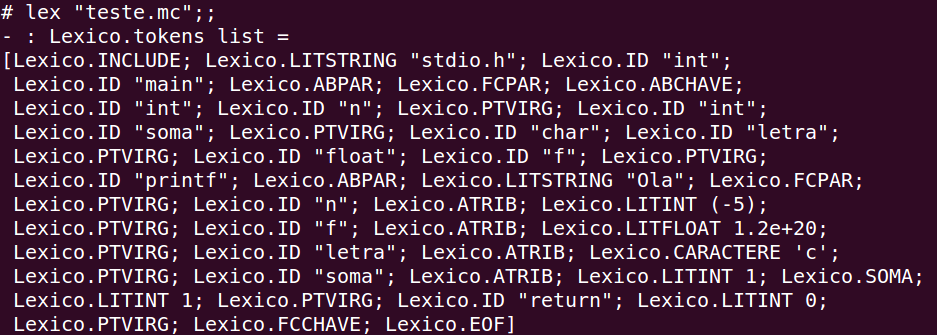
\includegraphics[scale=0.45]{imagens/lextestemc.png}
\end{figure}

\chapter{Analisador Sintático}

\section{Análise Sintática}

A análise sintática transforma um texto na entrada em uma estrutura de dados, em geral uma árvore, o que é conveniente para processamento posterior e captura a hierarquia implícita desta entrada. Através da análise léxica é obtido um grupo de tokens, para que o Analisador Sintático use um conjunto de regras para construir uma árvore sintática da estrutura.

Em termos práticos, por exemplo, pode também ser usada para decompor um texto em unidades estruturais para serem organizadas dentro de um bloco.

\section{Exemplo de Analisador Sintático LL(1)}

Nesta seção é mostrada a implementação de um exemplo de Analisador Sintático LL(1) para a seguinte gramática:
\begin{verbatim}
S -> XYZ

X -> aXb
X -> (vazio) 

Y -> cYZcX
Y -> d

Z -> eZYe
Z -> f
\end{verbatim}

Primeiro, construimos a tabela LL(1) e, em seguida, a tabela do Analisador Sintático.

\begin{table}
    \centering
    \begin{tabular}{c|c|c|c}
        & Anulável  & First     & Follow\cr
     S  & Não       & a, c, d   & \{ \}\cr
     X  & Sim       & a         & b, c, d, e, f\cr
     Y  & Não       & c, d      & e, f\cr
     Z  & Não       & e, f      & c, d
    \end{tabular}
    \caption{Tabela LL(1)}
    \centering
\end{table}
\begin{table}
    \centering
    \begin{tabular}{c|c|c|c|c|c|c}
        & a    & b          & c         & d         & e         & f\cr
    S   & XYZ  & -          & XYZ       & XYZ       & -         & -\cr
    X   & aXb  & (vazio)    & (vazio)   & (vazio)   & (vazio)   & (vazio)\cr  
    Y   & -    & -          & cYZcx     & d         & -         & -\cr
    Z   & -    & -          & -         & -         & eZYe      & f\cr
    \end{tabular}
    \caption{Tabela Analisador Sintático}
\end{table}

Com base nas tabelas, implementamos nossos arquivos em Ocaml "lexico.mll" e "sintatico.ml":

\lstinputlisting[caption={lexico.mll},label={arq:lexico2}] {codigos/AnalisadorSintaticoTeste/lexico.mll}

\lstinputlisting[caption={sintatico.ml},label={arq:sintatico}] {codigos/AnalisadorSintaticoTeste/sintatico.ml}

\section{Testando o Analisador Sintático LL(1)}

Primeiro compilamos o arquivo "lexico.mll" utilizando o comando:

\begin{terminal}
ocamllex lexico.mll
\end{terminal}

Gerando o arquivo "lexico.ml". Em seguida:

\begin{terminal}
ocamlc -c lexico.ml
\end{terminal}

Que irá gerar os binários "lexico.cmi" e "lexico.cmo".

Feito isso, invocamos o interpretador Ocaml:

\begin{terminal}
rlwrap ocaml
\end{terminal}

Importamos nosso arquivo do Analisador Sintático, "sintatico.ml":

\begin{terminal}
#use "sintatico.ml";;
\end{terminal}

E então invocamos a função de análise sintática chamada "parser" passando uma string de entrada como parâmetro:

\begin{terminal}
parser "abcdfcf";;
\end{terminal}

Que irá retornar uma resposta se a string de entrada pertence à gramática ou não. Nesse caso, a string "abcdfcf" pertence à nossa gramática usada no exemplo:

\begin{figure}[!h]
\centering
\caption{Analisador Sintático LL(1)} \label{fig:sintatico}
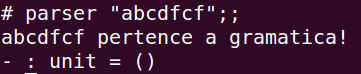
\includegraphics[scale=0.45]{imagens/sintatico.png}
\end{figure}

\section{Costruindo um Analisador Sintático LR(1) para MiniC}

Para construir o Analisador Sintático para a linguagem MiniC, utilizaremos a ajuda de uma ferramenta chamada Menhir.

\begin{terminal}
sudo apt-get install menhir
\end{terminal}

Menhir é um gerador de parser LR(1) para a linguagem de programacao OCaml. Ou seja, Menhir compila as especificações de uma gramática LR(1) para códio OCaml. Menhir foi projetado e implementado por François Pottier e Yann Régis-Gianas.

Um parser LR(1) é um parser LR(k) para k=1, ou seja, com um único terminal de "lookahead". O atributo especial deste parser é que todos os parsers LR(k), com k>1, podem ser transformados em um parser LR(1). Este pode lidar com todas as linguagens determinísticas livres de contexto. No passado, o parser LR(k) era evitado por causa de sua alta memória requerida, a favor de alternativas menos poderosas tais como LALR e o parser LL(1). Recentemente, entretanto, um "parser LR(1) mínimo", cujo espaço requerido é próximo aos parsers LALR, está sendo ofertado por boa parte dos geradores de parser. 

Como foi dito acima, Menhir compila as especificações de uma gramática LR(1) para código OCaml. As especificações da linguagem MiniC se encontram no arquivo "sintatico.mly":

\lstinputlisting[caption={sintatico.mly},label={arq:sintatico}] {codigos/AnalisadorSintatico/sintatico.mly}

Para compilar o arquivo "sintatico.mly" usando o menhir, utilize o comando:

\begin{terminal}
menhir -v "sintatico.mly"
\end{terminal}

Serão gerados o autômato finito determinístico para a linguagem e, caso haja conflitos na linguagem, um arquivo "conflicts" de log dos conflitos ocorridos. No caso de conflitos desloca/reduz, o Menhir escolhe uma opção arbitrariamente para cada conflito para gerar o AFD.

Após definir as especificações da nossa linguagem MiniC, escrevemos nossa Árvore Sintática Abstrata (AST).

Árvores sintáticas abstratas, assim como as árvore de análise sintática, são estruturas de dados em árvore que representam estruturas sintáticas de cadeias, de acordo com alguma gramática formal, porém os nós são diretamente valorados em seus símbolos terminais, não havendo portanto a representação das derivações por meio dos símbolos não terminais.

É uma representação abstrata (simplificada) da estrutura semântica de um código fonte escrito em uma certa linguagem de programação. Cada nó da árvore denota um construtor no código fonte. A sintaxe é abstrata no sentido que ela não representa cada detalhe que aparece na sintaxe real. Por exemplo, agrupar parênteses está implícito na estrutura da árvore, e uma construção sintática como um condicional SE cond ENTÃO expr pode ser denotada por um simples nó com suas ramificações.

O arquivo "ast.ml" contém as definições de nossa AST, que será gerada após a análise sintática de um código fonte.

\lstinputlisting[caption={ast.ml},label={arq:ast}] {codigos/AnalisadorSintatico/ast.ml}

Para testar o Analisador Sintático, definiremos funções de teste no arquivo "sintaticoCarregador.ml":

\lstinputlisting[caption={sintaticoCarregador.ml},label={arq:sintatico}] {codigos/AnalisadorSintatico/sintaticoCarregador.ml}

Também utilizaremos um arquivo ".ocamlinit" que nos ajudará a carregar e abrir os módulos necessários do Analisador no interpretador do OCaml:

\lstinputlisting[caption={.ocamlinit},label={arq:sintatico}] {codigos/AnalisadorSintatico/ocamlinit}

Para compilar todos os arquivos necessários, utilizaremos o "ocamlbuild" em conjunto com Menhir:

\begin{terminal}
ocamlbuild -use-menhir sintaticoCarregador.byte
\end{terminal}

Em seguida invocamos o interpretador OCaml:

\begin{terminal}
rlwrap ocaml
\end{terminal}

Chamamos a função de teste passando nosso arquivo fonte em MiniC "exs.mc":

\begin{terminal}
parse_arq "exs.mc";;
\end{terminal}

\lstinputlisting[caption={exs.mc},label={arq:sintatico}] {codigos/MiniC/exs.mc}\

Gerando a AST correspondente:

\begin{figure}[!h]
\centering
\caption{Árvore Sintática Abstrata (AST)} \label{fig:sintatico}
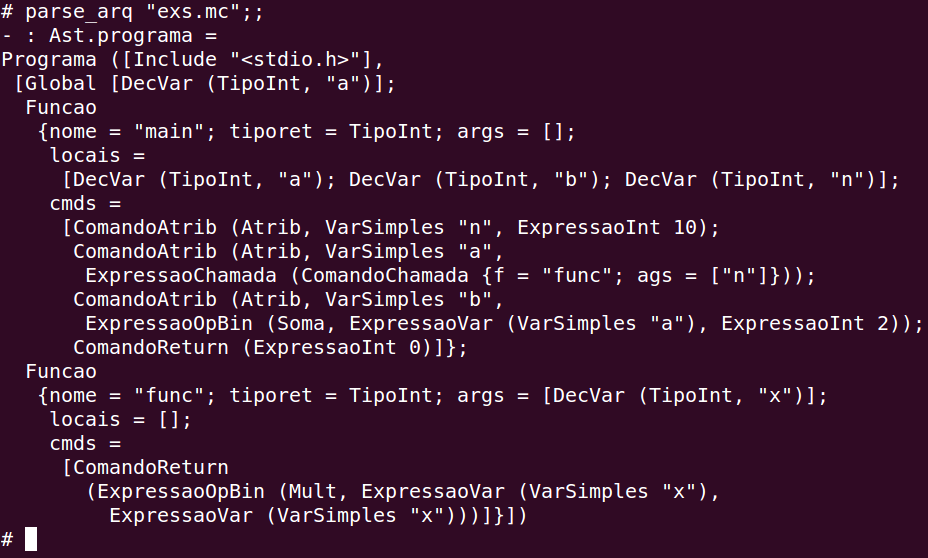
\includegraphics[scale=0.45]{imagens/exs.png}
\end{figure}

\section{Adicionando mensagens de erro}

Após concluirmos nosso Analisador Sintático, este ainda não é muito eficiente, pois não possui um mecanismo para detecção exata dos possíveis erros sintáticos e léxicos que podem ocorrer ao escrever nosso código fonte em MiniC.

Felizmente, a ferramenta Menhir possui uma opção de listar os possíveis erros gerados em nosso autômato do Analisador Sintático.

Utilizando o seguinte comando

\begin{terminal}
menhir -v --list-errors sintatico.mly > sintatico.messages
\end{terminal}

fazemos com que o menhir liste os possíveis erros de nossa gramática que possam ser encontrados ao gerar o autômato correspondente do nosso Analisador Sintático, listando-os para o arquivo "sintatico.messages".

Feito isso, teremos uma lista de erros em nosso arquivo e um exemplo que ilustra cada um, seguido de um espaço para adicionarmos as mensagens de erro correspondentes.

Após escrevermos todas as nossas mensagens de erro possíveis, utilizamos o menhir novamente para compilar as mesmas para o arquivo "erros.ml" que será utilizado em nosso arquivo "sintaticoCarregador.ml":

\begin{terminal}
menhir -v --list-errors sintatico.mly --compile-errors sintatico.messages > erros.ml
\end{terminal}

Em seguida adicionamos algumas linhas em nossos arquivos:

\begin{enumerate}
\item Em "lexico.mll":
\begin{verbatim}
exception Erro of string
\end{verbatim}

\item Em ".ocamlinit":
\begin{verbatim}
#use "topfind";;
#require "menhirLib";;
#load "erros.cmo";;
\end{verbatim}

\item Por último, alteraremos todo nosso arquivo "sintaticoCarregador.ml", adicionando o seguinte código:

\begin{verbatim}
open Printf
open Lexing
open Erros
open Ast

exception Erro_Sintatico of string
    
module S = MenhirLib.General (* Streams *)
module I = Sintatico.MenhirInterpreter

let posicao lexbuf =
    let pos = lexbuf.lex_curr_p in
    let lin = pos.pos_lnum
    and col = pos.pos_cnum - pos.pos_bol - 1 in
    sprintf "linha %d, coluna %d" lin col

(* [pilha checkpoint] extrai a pilha do autômato LR(1) contida em checkpoint *)

let pilha checkpoint =
  match checkpoint with
  | I.HandlingError amb -> I.stack amb
  | _ -> assert false (* Isso não pode acontecer *)

let estado checkpoint : int =
  match Lazy.force (pilha checkpoint) with
  | S.Nil -> (* O parser está no estado inicial *)
     0
  | S.Cons (I.Element (s, _, _, _), _) ->
     I.number s

let sucesso v = v

let falha lexbuf (checkpoint : Ast.programa I.checkpoint) =
  let estado_atual = estado checkpoint in
  let msg = message estado_atual in
  raise (Erro_Sintatico (Printf.sprintf "%d - %s.\n"
                                      (Lexing.lexeme_start lexbuf) msg))

let loop lexbuf resultado =
  let fornecedor = I.lexer_lexbuf_to_supplier Lexico.token lexbuf in
  I.loop_handle sucesso (falha lexbuf) fornecedor resultado



let parse_com_erro lexbuf =
  try
    Some (loop lexbuf (Sintatico.Incremental.programa lexbuf.lex_curr_p))
  with
  | Lexico.Erro msg ->
     printf "Erro lexico na %s:\n\t%s\n" (posicao lexbuf) msg;
     None
  | Erro_Sintatico msg ->
     printf "Erro sintático na %s %s\n" (posicao lexbuf) msg;
     None

let parse s =
  let lexbuf = Lexing.from_string s in
  let ast = parse_com_erro lexbuf in
  ast

let parse_arq nome =
  let ic = open_in nome in
  let lexbuf = Lexing.from_channel ic in
  let ast = parse_com_erro lexbuf in
  let _ = close_in ic in
  ast
\end{verbatim}
\end{enumerate}

Para compilar nosso novo programa utilizaremos o seguinte:

\begin{terminal}
ocamlbuild -use-ocamlfind -use-menhir -menhir "menhir --table" -package menhirLib sintaticoCarregador.byte
\end{terminal}

Em seguida:

\begin{terminal}
rlwrap ocaml
\end{terminal}

Agora, ao invocarmos nossa nova função parse passando um código fonte com erro sintático, a mesma nos retorna o devido local do erro e uma mensagem correspondente.

Vamos tomar o seguinte código como exemplo:

\lstinputlisting[caption={exserro.mc},label={arq:sintatico}] {codigos/MiniC/exserro.mc}

Invocando parse em "exserro.mc" obtemos a seguinte mensagem:

\begin{figure}[!h]
\centering
\caption{Mensagem de Erro Sintático} \label{fig:sintatico}
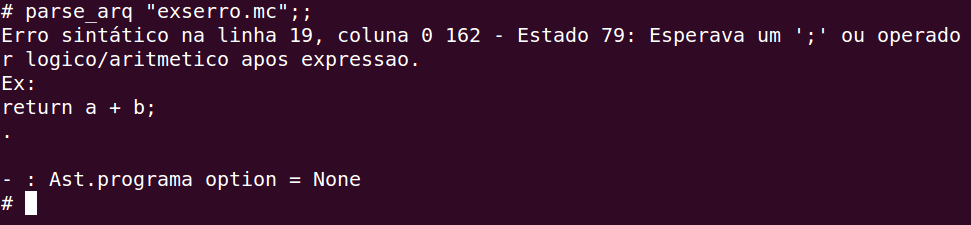
\includegraphics[scale=0.5]{imagens/exserro.png}
\end{figure}

\chapter{Analisador Semântico}

\section{Análise Semântica}

Análise semântica é a terceira fase da compilação onde se verificam os erros semânticos, (por exemplo, fazer a divisão de um número inteiro por outro numero float, na linguagem C padrão ANSI)) no código fonte e coletam-se as informações necessárias para a próxima fase da compilação, que é a geração de código objeto.

A análise semântica trata a entrada sintática e transforma-a numa representação mais simples e mais adaptada a geração de código. Esta camada do compilador fica igualmente encarregada de analisar a utilização dos identificadores e de ligar cada uma delas a sua declaração. Nesta situação verificar-se que o programa respeita as regras de visibilidade e de porte dos identificadores. Nesta fase é também esperado que no processo da compilação verifique que cada expressão definida tenha um tipo adequado conforme as regras próprias da linguagem.

O objetivo da análise semântica é trabalhar nesse nível de inter-relacionamento entre partes distintas do programa. As tarefas básicas desempenhada durante a análise semântica incluem a verificação de tipos, a verificação do fluxo de controle e a verificação da unicidade da declaração de variáveis. 

\section{Construindo um Analisador Semântico para MiniC}

Para construirmos um Analisador semântico, precisamos definir um verificador de tipos para realizar a verificação dos tipos declarados de variáveis e funções declaradas em nosso programa fonte através de regras de inferência. Nas regras de inferência, as variáveis são agrupadas em um ambiente, também chamado de contexto. O ambiente é uma tabela de símbolos que mapeia uma variável para seu tipo.

Nosso ambiente será definido no arquivo "tabsim.ml":

\lstinputlisting[caption={tabsimb.ml},label={arq:semantico}] {codigos/AnalisadorSemantico/tabsimb.ml}

Já o verificador de tipos para variáveis e funções, bem como as regras de inferência e funções para exibição de mensagens de erro semântico são mostradas a seguir:

\lstinputlisting[caption={semantico.ml},label={arq:semantico}] {codigos/AnalisadorSemantico/semantico.ml}

\section{Testando o Analisador Semântico}

Primeiramente, escreveremos um arquivo com funções para teste.

\lstinputlisting[caption={semanticoTest.ml},label={arq:semantico}] {codigos/AnalisadorSemantico/semanticoTest.ml}

Em seguida, utilizamos um arquivo fonte em MiniC para testarmos nosso Analisador semântico.

\lstinputlisting[caption={exsemantico.mc},label={arq:semantico}] {codigos/AnalisadorSemantico/ex.c}

Compilamos nossos arquivos em OCaml:

\begin{terminal}
ocamlbuild -use-ocamlfind -use-menhir -menhir "menhir --table" -package menhirLib semanticoTest.byte
\end{terminal}

Invocamos o interpretador:

\begin{terminal}
rlwrap ocaml
\end{terminal}

Finalmente, chamamos a funcao verificatipos, passando nosso exemplo como parâmetro:

\begin{terminal}
verifica_tipos "exsemantico.mc"
\end{terminal}

A função irá retornar uma AST com os tipos correspondentes para cada função, variável e comando declarado:
\begin{verbatim}
- : Tast.expressao Ast.programa * Ambiente.t =
(Programa ([Bib "stdio.h"],
  [Funcao
    {nome =
      ("soma",
       {Lexing.pos_fname = ""; pos_lnum = 3; pos_bol = 20; pos_cnum = 24});
     tipReturn = TipoInt;
     args =
      [(("n1",
         {Lexing.pos_fname = ""; pos_lnum = 3; pos_bol = 20; pos_cnum = 33}),
        TipoInt);
       (("n2",
         {Lexing.pos_fname = ""; pos_lnum = 3; pos_bol = 20; pos_cnum = 41}),
        TipoInt)];
     locais = [];
     cmds =
      [CmdReturn
        (Some
          (Tast.ExpOpBin ((Soma, TipoInt),
            (Tast.ExpVar
              (VarSimples
                ("n1",
                 {Lexing.pos_fname = ""; pos_lnum = 5; pos_bol = 47;
                  pos_cnum = 57}),
              TipoInt),
             TipoInt),
            (Tast.ExpVar
              (VarSimples
                ("n2",
                 {Lexing.pos_fname = ""; pos_lnum = 5; pos_bol = 47;
                  pos_cnum = 62}),
              TipoInt),
             TipoInt))))]};
   Funcao
    {nome =
      ("main",
       {Lexing.pos_fname = ""; pos_lnum = 8; pos_bol = 69; pos_cnum = 73});
     tipReturn = TipoInt; args = [];
     locais =
      [DecVar
        (("a",
          {Lexing.pos_fname = ""; pos_lnum = 10; pos_bol = 82; pos_cnum = 89}),
        TipoInt);
       DecVar
        (("b",
          {Lexing.pos_fname = ""; pos_lnum = 10; pos_bol = 82; pos_cnum = 92}),
        TipoInt);
       DecVar
        (("resultado",
          {Lexing.pos_fname = ""; pos_lnum = 11; pos_bol = 95;
           pos_cnum = 102}),
        TipoInt);
       DecVar
        (("i",
          {Lexing.pos_fname = ""; pos_lnum = 12; pos_bol = 113;
           pos_cnum = 120}),
        TipoInt)];
     cmds =
      [CmdAtrib
        (Tast.ExpVar
          (VarSimples
            ("a",
             {Lexing.pos_fname = ""; pos_lnum = 14; pos_bol = 124;
              pos_cnum = 127}),
          TipoInt),
        Tast.ExpInt (10, TipoInt));
       CmdAtrib
        (Tast.ExpVar
          (VarSimples
            ("b",
             {Lexing.pos_fname = ""; pos_lnum = 15; pos_bol = 135;
              pos_cnum = 138}),
          TipoInt),
        Tast.ExpInt (5, TipoInt));
       CmdAtrib
        (Tast.ExpVar
          (VarSimples
            ("resultado",
             {Lexing.pos_fname = ""; pos_lnum = 17; pos_bol = 149;
              pos_cnum = 152}),
          TipoInt),
        Tast.ExpChamada ("soma",
         [Tast.ExpVar
           (VarSimples
             ("a",
              {Lexing.pos_fname = ""; pos_lnum = 17; pos_bol = 149;
               pos_cnum = 169}),
           TipoInt);
          Tast.ExpVar
           (VarSimples
             ("b",
              {Lexing.pos_fname = ""; pos_lnum = 17; pos_bol = 149;
               pos_cnum = 172}),
           TipoInt)],
         TipoInt));
       CmdPuts
        (Tast.ExpVar
          (VarSimples
            ("resultado",
             {Lexing.pos_fname = ""; pos_lnum = 19; pos_bol = 177;
              pos_cnum = 185}),
          TipoInt));
       CmdReturn (Some (Tast.ExpInt (0, TipoInt)))]}]),
 <abstr>)
\end{verbatim}

Ao introduzirmos um erro semântico no arquivo fonte na linha 14, atribuindo uma string à variável int a, uma mensagem de erro será exibida:

\begin{figure}[!h]
\centering
\caption{Mensagem de Erro Semântico} \label{fig:semantico}
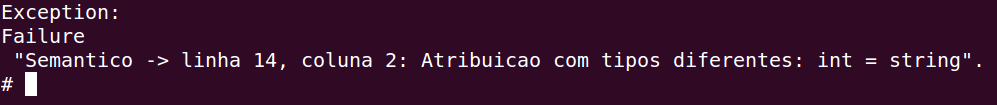
\includegraphics[scale=0.5]{imagens/errosemantico.png}
\end{figure}

\chapter{Interpretador}
Interpretadores são programas de computador que leem um código fonte de uma linguagem de programação interpretada e o converte em código executável. Seu funcionamento pode variar de acordo com a implementação. Em alguns casos, o interpretador lê linha-por-linha e converte em código objeto (ou bytecode) à medida que vai executando o programa e, em outros casos, converte o código fonte por inteiro e depois o executa.

\section{Construindo um Interpretador}
Nessa última etapa, construiremos um interpretador funcional para MiniC que utilizará os módulos Léxico, Sintático e Semântico para interpretar o código fonte e gerar os resultados necessários.

Para isso, como nas etapas anteriores, definimos nosso Interpretador:

\lstinputlisting[caption={interprete.ml},label={arq:interprete}] {codigos/Interpretador/interprete.ml}

As funções para teste:
\lstinputlisting[caption={interpreteTeste.ml},label={arq:interprete}] {codigos/Interpretador/interpreteTeste.ml}

Invocamos o interpretador OCaml:

\begin{terminal}
rlwrap ocaml
\end{terminal}

Compilamos nossos arquivos utilizando:

\begin{terminal}
ocamlbuild -use-ocamlfind -use-menhir -menhir "menhir --table" -package menhirLib interpreteTeste.byte
\end{terminal}

Finalmente, chamamos a função interprete e passamos nosso arquivo fonte como parâmetro.\\\\

A seguir, são mostrados alguns exemplos de programas e suas respectivas saídas:

\begin{figure}[!h]
\centering
\caption{Fatorial} \label{fig:fatorial}
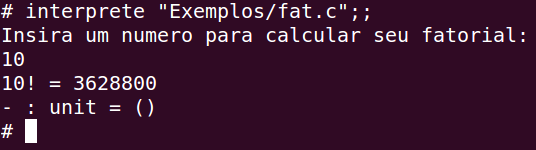
\includegraphics[scale=0.5]{imagens/fat.png}
\end{figure}

\begin{figure}[!h]
\centering
\caption{Fibonacci} \label{fig:fibonacci}
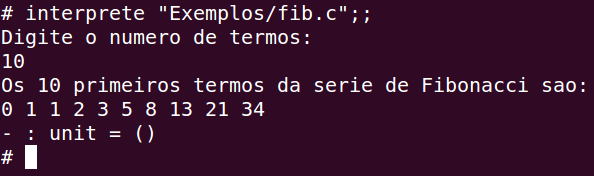
\includegraphics[scale=0.5]{imagens/fib.png}
\end{figure}

\begin{figure}[!h]
\centering
\caption{M.D.C.} \label{fig:mdc}
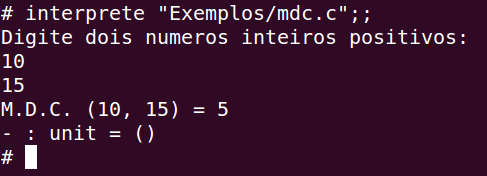
\includegraphics[scale=0.5]{imagens/mdc.png}
\end{figure}

\begin{figure}[!h]
\centering
\caption{Crivo de Eratóstenes} \label{fig:fatorial}
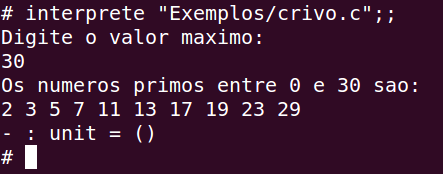
\includegraphics[scale=0.5]{imagens/crivo.png}
\end{figure}

\begin{enumerate}
\item{Fatorial}
\lstinputlisting[caption={fat.c},label={arq:Fatorial}] {codigos/Interpretador/fatrec.c}
\item{Série de Fibonacci}
\lstinputlisting[caption={fib.c},label={arq:Fibonacci}] {codigos/Interpretador/fibrec.c}
\item{Máximo Divisor Comum - MDC}
\lstinputlisting[caption={mdc.c},label={arq:mdc}] {codigos/Interpretador/mdc.c}
\item{Crivo de Eratóstenes}
\lstinputlisting[caption={crivo.c},label={arq:crivo}] {codigos/Interpretador/crivo.c}
\end{enumerate}

\chapter{Bibliografia}
\url{https://ocaml.org/docs/}\\

\url{http://www2.lib.uchicago.edu/keith/ocaml-class/compiling.html}\\

\url{https://pt.wikipedia.org/wiki/Análise_léxica}\\

\url{https://pt.wikipedia.org/wiki/Análise_sintática_(computação)}\\

\url{https://pt.wikipedia.org/wiki/Análise_semântica}\\

\url{https://pt.wikipedia.org/wiki/Interpretador}
\end{document} 